\documentclass[12pt]{article}

\usepackage[utf8]{inputenc}
\usepackage[margin=1in]{geometry}
\usepackage{setspace}
\usepackage{graphicx}
\usepackage{url}
\usepackage{pdfpages}

\doublespacing

\title{Close Reading of a Page:\\
``She's Only a Girl'': Judgment, Shame, and Internalized Gender in Alice Munro's \textit{Boys and Girls}}

\author{%
  Ma Toan Bach\\
  LSO100KCC\\
  Close Reading of a Page
}

\date{}

\begin{document}

\maketitle

\section{Introduction}
This essay offers a close reading of page 16 of the downloaded PDF of Alice Munro's \textit{Boys and Girls}, focusing on the final dinner-table exchange. Munro's narrator learns that ``girl'' is not a neutral description but a social judgment. Here, the father's line, ``She's only a girl,'' does not simply excuse her tears; it closes the conversation by turning her act into a gender explanation. The narrator's final response---``Maybe it was true''---shows how quickly that explanation can begin to feel like self-knowledge (Munro, 1968, p.~16).

\section{Public Gaze and Embodied Shame}
The scene begins with exposure. After Laird reports that his sister ``just open' it up / and Flora ran out,'' the father asks, ``Is that right?'' (Munro, 1968, p.~16). Munro then pivots from action to surveillance: ``Everybody at the table was looking at me.'' The narrator's body registers the moment before her mind can explain it; she nods while ``swallowing food with great difficulty,'' and ``tears flooded'' her eyes ``to [her] shame'' (Munro, 1968, p.~16). ``Shame'' is the key word: the tears are treated as evidence that she has violated an expectation she cannot defend.

The phrasing ``To my shame'' also suggests retrospection. The narrator does not simply report that she cried; she evaluates the crying as a failure, adopting the judgment that the table will soon articulate. Even before the father speaks, Munro shows the narrator beginning to police herself.

\section{Authority, Disgust, and the Demand for an Explanation}
The father's authority shows up as contempt, not outrage: he makes ``a curt sound of disgust'' and asks, ``What did you do that for?'' (Munro, 1968, p.~16). The question demands a reason, but the narrator cannot produce one: ``I didn't answer.'' She sets down her fork and ``waited to be sent from the table,'' ``still not looking up'' (Munro, 1968, p.~16). The posture reads like self-sentencing---as if shame has already pushed her into the role of the guilty.

That expectation of punishment matters because it frames what follows. The narrator anticipates consequences for an action; the family instead supplies a category that makes consequences unnecessary. Munro shifts the scene from discipline (what you did) to definition (what you are).

Because the narrator's earlier action at the gate cannot be openly explained, the dinner-table scene turns that action into a judgment about gender rather than a discussion of choice.

\section{Communal Pressure and Enforcement}
Munro slows the scene with a pause: ``For some time nobody said anything'' (Munro, 1968, p.~16). The silence holds the narrator at the table and turns the moment into a shared evaluation rather than a private feeling. When speech returns, it returns as interpretation.

Laird breaks the silence by naming the visible: ``She's crying'' (Munro, 1968, p.~16). The line is ``matter-of-fact,'' and that flatness matters; he turns her emotion into the central ``fact'' of the situation. He does not need to argue about the gate anymore because the story of the moment has become the story of her tears.

\section{The Verdict: Dismissal Disguised as Mercy}
The father responds, ``Never mind,'' speaking ``with resignation, even good humor'' (Munro, 1968, p.~16). The narration immediately clarifies what that tone accomplishes: the words ``absolved and dismissed'' her ``for good.'' His final explanation---``She's only a girl''---reduces her act to essence (Munro, 1968, p.~16). ``Only'' is the lever: it turns a consequential choice into something too small to confront seriously.

The line also masquerades as mercy. If she is ``only'' a girl, she is spared the full weight of blame, but she is also denied the dignity of being taken seriously. Munro marks the cost as permanent: she is dismissed ``for good'' (Munro, 1968, p.~16).

The doubled phrasing ``absolved and dismissed'' is especially sharp. ``Absolved'' sounds like forgiveness, but it also implies that her action is not being treated as a moral decision worth engaging; it is explained away. ``Dismissed'' then seals the social consequence: she is removed from the sphere of meaningful responsibility. Even the ``good humor'' participates in this mechanism. It keeps the table comfortable, encouraging everyone to accept the verdict as commonsense rather than cruelty.

\section{Internalization and the Softness of ``Maybe''}
The last sentences pull the verdict inward: ``I didn't protest that, even in my heart. Maybe it was true'' (Munro, 1968, p.~16). The narrator does not argue against the label; she considers it. ``Maybe'' is both hesitation and entry point: it shows how an external judgment can become plausible from the inside, especially when shame has already made resistance feel unspeakable.

Munro leaves ``maybe'' open-ended: it can sound like resignation, like stunned agreement, or like the first step toward self-awareness about how power works. The ambiguity is the point. The story ends not with a lesson delivered, but with a mind reshaped.

\section{Conclusion}
This page shows Munro's method of making gender feel inevitable: not through lectures, but through gaze, silence, and a verdict delivered as ``good humor.'' By ending on ``Maybe it was true,'' Munro shows the final stage of socialization: the moment when dismissal starts to sound like description (Munro, 1968, p.~16).

\begin{thebibliography}{00}

\bibitem{Munro1968pdf}
Munro, A. (1968). \textit{Boys and girls} [PDF]. Retrieved May 27, 2026, from \url{https://jerrywbrown.com/wp-content/uploads/2014/02/Boys-and-Girls-by-Alice-Munro.pdf}

\end{thebibliography}

\clearpage
\appendix
\section*{Selected Page (p.~16)}
\includepdf[pages=16]{Boys-and-Girls-by-Alice-Munro.pdf}

\end{document}
